
 

%---- Begin PDF metadata ---------%
\usepackage{hyperref}
\hypersetup{%
	pdftitle={URDAD as Quality-Driven Process},%
	pdfauthor={Fritz Solms, Stefan Gruner and Cuen Edwards},%
	pdfsubject={},%
	pdfkeywords={URDAD, Quality driver}%
}
%---- End PDF metadata ---------%

% --- Graphics support ----%
\usepackage{graphicx}

% ---- Ticking clock for presentation ---%
% Duration of presentation = 20 minutes, change color at 50% and 80% of time, update clock every 29 seconds
% This is used in conjunction with \tdtime, \crono or \cronominutes
\usepackage[font=Times,timeinterval=29, timeduration=20.0, timedeath=0, fillcolorwarningsecond=white!60!yellow,timewarningfirst=50,timewarningsecond=80]{tdclock}


%--------------- Begin Beamer styling  -------------%

\usetheme{Berkeley}
% default 
%	AnnArbor | Antibes | Bergen |
%	Berkeley | Berlin | Boadilla |
%	boxes | CambridgeUS | Copenhagen |
%	Darmstadt | default | Dresden |
%	Frankfurt | Goettingen |Hannover |
%	Ilmenau | JuanLesPins | Luebeck |
%	Madrid | Malmoe | Marburg |
%	Montpellier | PaloAlto | Pittsburgh |
%	Rochester | Singapore | Szeged |
%	Warsaw

\setbeamertemplate{background canvas}{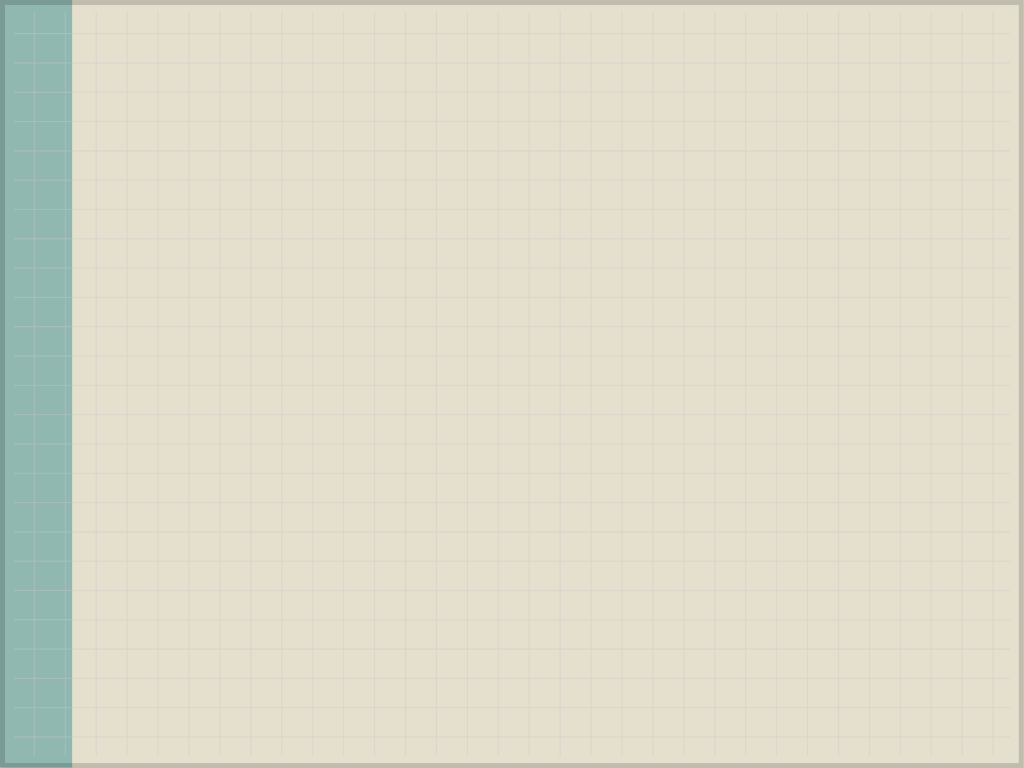
\includegraphics
	[width=\paperwidth,height=\paperheight]{background.png}}
\setbeamercolor{structure}{fg=DarkSlateGray} 
\setbeamercolor{normal text}{fg=Black} 
%\setbeamercolor{alerted text}{fg=Crimson} 
%\setbeamercolor{alerted text}{fg=DarkRed} 
\setbeamerfont{structure}{series=\bfseries} 
%\setbeamersize{text margin left=10mm}

% To insert outline slides before every section
%\AtBeginSection[]
%{
%   \begin{frame}
%       \frametitle{Outline}
%       \tableofcontents[currentsection]
%   \end{frame}
%}

%--------------- End Beamer styling  -------------%

\usepackage{color}
\usepackage{listings}
\lstdefinelanguage{urdad}
{
keywords=
  {Model,ResponsibilityDomain,Query,Constraint,QualityConstraint,FunctionalRequirements,receiving,yielding,
  StateConstraint,stateAssessmentProcess,InverseConstraint,inverseOf,AndConstraint,AND,OrConstraint,OR,
  XorConstraint,XOR,from,to,many,BasicDataType,DataStructure,is,abstract,has,Variable,ofType,Constant,
  ValueOf,Exception,attribute,identification,identifying,association,linking,aggregate,component,
  QualityRequirement,requiredBy,constraint,with,constructedUsing,ResultConstraint,PreCondition,
  raises,checks,PostCondition,ensures,use,toAddress,if,ServiceContract,undoneUsing,Request,Result,
  Service,realizes,doSequential,choice,else,doConcurrent,blocking,Concurrency,wait,until,create,set,
  equalTo,add,remove,requestService,on,raiseException,returnResult,while,do,forAll,Note},%
sensitive=true,%
alsoletter={\$},%
comment=[l]{\#},%
string=[b]",%
string=[b]'%
}

%\definecolor{OliveGreen}{cmyk}{0.64,0,0.95,0.40}
%\definecolor{CadetBlue}{cmyk}{0.62,0.57,0.23,0}
\definecolor{lightgray}{gray}{0.9}
\lstset{
language=urdad,  
basicstyle=\ttfamily\tiny,
keywordstyle=\itshape\color{blue},
%keywordstyle=\color{blue},        % Keywords font ('*' = uppercase)
commentstyle=\color{gray},           
numbers=left,                           % Line nums position
numberstyle=\tiny,                      % Line-numbers fonts
stepnumber=1,                           % Step between two line-numbers
numbersep=5pt,                          % How far are line-numbers from code
backgroundcolor=\color{lightgray}, % Choose background color
frame=none,                             % A frame around the code
tabsize=2,                              % Default tab size
captionpos=b,                           % Caption-position = bottom
breaklines=true,                        % Automatic line breaking?
breakatwhitespace=false,                % Automatic breaks only at whitespace?
showspaces=false,                       % Dont make spaces visible
showtabs=false,                         % Dont make tabls visible
columns=flexible,                       % Column format
%morekeywords={__global__, __device__},  % CUDA specific keywords
}


\begin{document}

\conferenceinfo{SAICSIT}{'11, October 3-5, Cape Town, South Africa}
\CopyrightYear{2011} 
\crdata{}

\title{A Domain-Specific Language for URDAD Based Requirements Elicitation}

%\frontmatter          % for the preliminaries
%\pagestyle{headings}  % switches on printing of running heads
%\title{A Domain-Specific Language for URDAD Based Requirements Elicitation}
%\titlerunning{DSL for URDAD}  % abbreviated title (for running head)

\numberofauthors{1} 
\author{
\alignauthor Fritz Solms, Craig Edwards, Alexander Paar, Stefan Gruner\\
			 \affaddr{Department of Computer Science}\\
       \affaddr{University of Pretoria}\\
       \affaddr{South Africa}\\
       \email{fritz@solms.co.za}
}

\maketitle

%Now the list of todo's could be inserted by using the command
%\listoftodos

\begin{abstract}
Use-Case Responsibility-Driven Analysis and Design (URDAD) is a service-oriented software analysis and design methodology. It is used by requirements engineers to develop technology-neutral, semi-formal platform-indepen\-dent models (PIM) within the OMG's MDA. In the past, URDAD models were denoted in UML. However, that was tedious and error-prone. The resulting models were often of rather poor quality. In this paper we introduce and discuss a new Domain-Specific Language (DSL) for URDAD. Its meta model is consistent and satisfiable. We show that URDAD DSL specifications are simpler and allow for more complete service contract specifications than their corresponding UML expressions. They also enable traceability and test case generation.
\end{abstract}


\keywords{Model Driven Development, Domain Specific Language, Meta Model, Service Orientation, Requirements Engineering, Platform Independent Model}
 
\section{Introduction}
Insufficiency in requirements engineering is still regarded as a root cause of poor software quality. This is due to various factors, both human and technological, including vague specification languages with only informally defined semantics. Insufficient language support for \emph{layered} specifications (i.e., decompositional system descriptions at different levels of granularity), leads software developers to making wrong presumptions about lower level requirements \cite{espana_evaluating_2009}. Tool support for the validation of requirements specifications, or for the automatic extraction of test cases from them, is also still weak \cite{bashardoust-tajali_extracting_2008}.

Model-Driven Engineering (MDE) \cite{schmidt_model_2006} aims at solving some of those problems by using modelling languages with well defined semantics, by requiring primary models to be domain models, not technical models \cite{asnina_computation_2010} and by providing tool support for MDE processes. Consequently, technology-neutral domain models are developed by requirements specialists, not by technical experts \cite{asnina_computation_2010}.

\emph{URDAD}, the Use-Case Responsibility-Driven Analysis and Design methodology \cite{fritz_solms_technology_2007} supports MDE in a service-oriented way \cite{solms_urdad_2010}. It is used by requirements specialists to develop and validate technology-neutral requirements models. URDAD models are thus Platform-Independent Models (PIM) in the Model-Driven Architecture (MDA) context \cite{solms_urdad_2010}. For each level of granularity the method leads to testable service contracts and for non-leaf services a technology neutral process realizing the service contract through the use of lower level services. Higher-level services are thus a functional composition of lower-level services, similar to the classical DFD technique \cite{demarco_tom_structured_1978}, with the levels of granularity decoupled through service contracts.

Requirements engineers have traditionally used the Unified Model Language (UML) to encode URDAD models. UML was a reasonable choice for this purpose because of its tool-supported use in the software industry. However, UML is an object oriented modeling language which is not conceptually aligned with a service oriented approach where stateless services are always assembled form lower level stateless services. On the one side it allows for a higher level services are assembled does not support many of the concepts required by the URDAD methodology explicitly and allows for a wide variety of model structures, most of which would not comply to the services-oriented structure of an URDAD model and on the other side it does not explicitly support many of the concepts required by URDAD. For example, the concept of a responsibility domain, a stakeholder, are not explicitly supported. Indeed, a specific UML \emph{profile} could be used to restrict the use of UML according to URDAD's intentions and at the same time introduce explicitly concepts required by URDAD. In practice, however, such a UML profile would contain an excessive number of metamodel constraints ensuring that a UML model complies structurally to a service-oriented URDAD model.

In this paper we present a new domain-specific language (DSL) for the domain of technology-neutral service-orien\-ted requirements modelling. Our new URDAD DSL is described in terms of a MOF/EMOF meta model. This makes it amenable to MDA tool suites for model transformations, as well as the generation of concrete textual and diagrammatic syntaxes with tool support \cite{gronback_model_2008}. To this end we analyse theoretically the modelling constructs required by URDAD. We elucidate and critically assess the URDAD meta model, and we propose a concrete textual syntax for an URDAD DSL. A Description Logics (DL)-based representation of the URDAD meta model is derived from the MOF/EMOF meta model in order to show its consistency and satisfiability.

Consequently we argue (also w.r.t. related work) that the URDAD DSL has two main advantages over the use of an URDAD UML profile. The language is considerably simpler than the UML and, with appropriate tool support, is expected to simplify the process through which requirements engineers can build high-level, technology-neutral models. Our new DSL enforces the structure required for a valid URDAD model, thereby requiring only a rather small and simple set of meta model constraints at the basis of tool-supported model validation. In addition the URDAD DSL provides better support for specifying service contracts within a service-oriented approach.



\section{Overview of the URDAD methodology \label{sec:urdadMethodology}}

URDAD as a methodology generating the requirements model

URDAD is an algorithmic, semi-formal methodology for eliciting and capturing service/use case requirements and technology neutral business process designs\cite{solms_urdad_2010}. 
TODO: REWRITE FOLLOWING PART OF PARAGRAPH
 The methodology recursively decomposes cohesive units of functional requirements into lower level functional requirements until the functional requirements are
fully specified in terms of well understood pieces of functionality.

Services are recursively decomposed until the lowest level services which are services sourced from the environment (e.g. operating system, frameworkd, off-the shelf solutions and services sourced from external service providers). These low level provided by the environment are treated as atomic services.

The process is an iterative process, iterating across levels of granularity. At each level of granularity the required functionality is decomposed into cohesive lower level functional units called services. The required logic for assembling the higher level functionality/service from lower level services is specified in a process.

The steps at any level of granularity include
\begin{enumerate}
 \item lower level {functional requirements elicitation}
 
Decompose the higher level functional requirement (service) into lower level functional requirements required by different stake holders.
 \item Specify the services contract for the higher level service including the pre- and post-conditions, data structures for the result and the quality requirements
 \item 
\end{enumerate}

Discuss recursive nature of URDAD, i.e. how URDAD can be used to design itself but refer to quality paper - feed that into quality paper.



\section{The URDAD metamodel \label{sec:metamodel}}

A metamodel contains the ``logical information model that specifies the modeling elements used within another (or the same) modeling notation
metamodel'' \cite{_ieee_2003}. The URDAD metamodel provides the modeling constructs required required by the URDAD methodology to store the requirements for a service/use case and the technology neutral design of a business process realizing these requirements. 

For practicality reasons, the semantics has been encoded EMOF/Ecore instead of {\em Web Ontology Language}, OWL\cite{}. It is motivated by the technology support for developing a concrete textual and graphical syntax for the DSL \cite{emfText,xText}, the support for model-to-model \cite{QVT relational, QVT operational, ,...} and model-to-text transformations \cite{model2text} and the availability of OCL as a constraint language \cite{OCL} for querying model instances and for specifying constraints at both, the metamodel and model levels. Mappings between these two technologies can be readily performed \cite{staab_model_2010}. A transformation to OWL facilitates reasoning services like consistency and completeness assessment.

The URDAD metamodel provides a minimalistic set of modeling constructs for services oriented analysis and design. It facilitates the recursive decomposition of service requirements into lower level services requirements with pre- and post-conditions as well as quality requirements for each service and the data structure specifications for the inputs and outputs and the process specification on how a service is orchestrated across lower level services.

The URDAD metamodel has been strongly influenced by the Unified Modeling Language, UML, in the areas of data structure specification and by service-oriented process specification languages like the Business Process Execution Language, BPEL, in the areas of process specification. 
It enforces assembly of higher level stateless services from lower level stateless services with the leaf services sourced from the environment (e.g.\ from the programming language, libraries, frameworks and automated and non-automated external service providers). 

The URDAD DSL is, however, a fraction of the size of the UML, yet adds some core concepts required by the URDAD methodologyCore additions include the following:
\begin{itemize}
  \item Explicit modeling constructs for specifying a services contract with pre- and post-conditions and quality requirements.
  \item The ``requiredBy'' linkage between requirements and stake holders who require these.
  \item Within a specific process specification for a service realizing a services contract, the URDAD DSL introduces the the linkage between functionality (services) and the requirements they are meant to address. 
  \item The Object Constraint Language (OCL) is generally used to specify constraints across object graphs. the URDAD DSL adds the constructs for defining a process to obtain the required information in order to assess the prost-conditions.
  \item The URDAD DSL adds the concept of a responsibility domain which represents an abstract role which may have requirements and may provide services. A responsibility domain also provides the packaging construct for the language.
  \item The specification of exceptions for pre-conditions.
  \item Enforcing that a service either yields the result or notifies the user that the service is not provided due to a pre-condition not having been met.
  \item Enforcing for each service request and result classes which are specific to that service.
\end{itemize}

%--------------------------

\subsection{URDAD-DSL core}

The core modules introduces the concept of the model, model elements and responsibility domains, expressions and annotations. Most of these are self-explanatory. Responsibility domains represent two important aspects within an URDAD model. They are primarily used to depict the roles or stakeholders that have  a direct or indirect interest in the service requirements that are being modelled. Secondly, they introduce the concept of packaging, where model elements belonging to these domains are associated with a unique name space. 

\begin{figure}
  \centering
  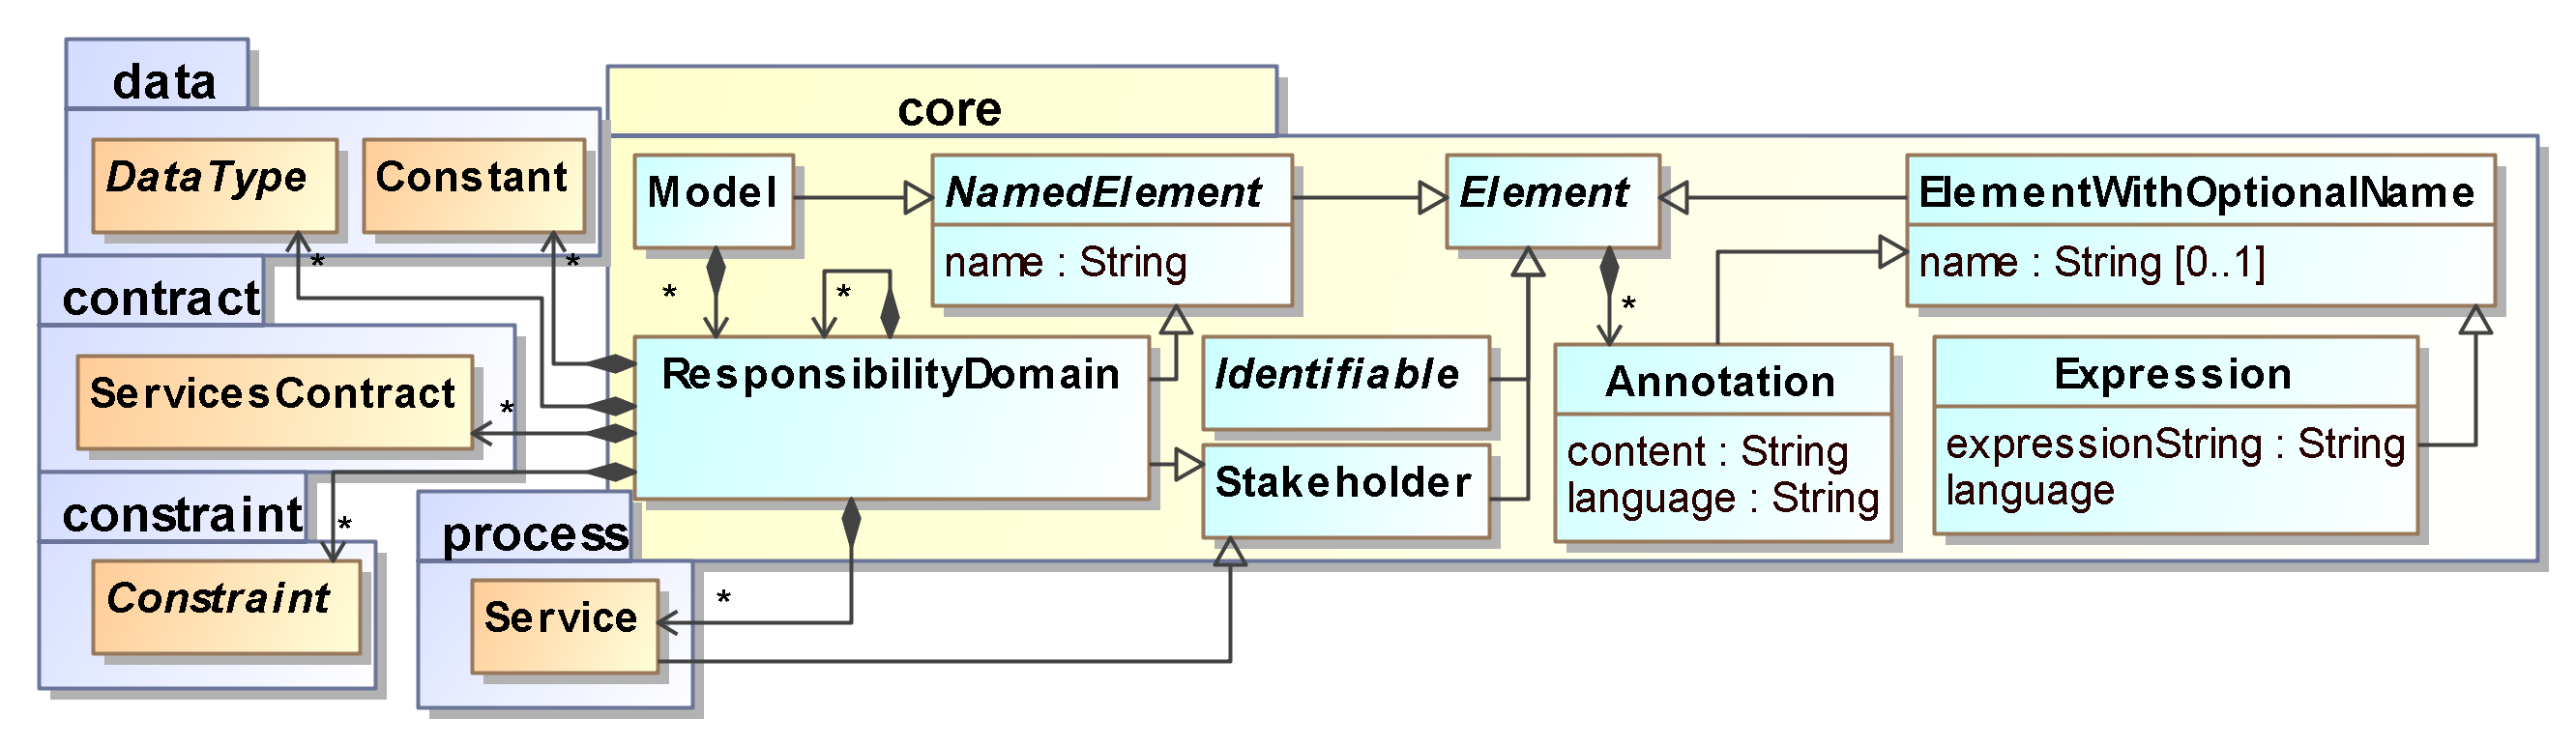
\includegraphics{core}
  \caption{The core elements of URDAD}
  \label{fig:metamodel}
\end{figure}

%--------------------------

\subsection{Constraints}

The Object-Constraint Language (OCL) has become the de-facto standard for specifying constraints across object graphs \cite{}. However, in a services oriented approach and in the context of reusable, parametrized constraints, OCL alone is insufficient.
Reusable constraints require support for binding parameters. For example, one might have a constraint that a person is registered. This constraint can be used in the context of pre-conditions for certain services and is most likely a post-condition for the registration service itself. However, the person identifier would have to be passed as a parameter to the constraint if the constraint is to be widely reusable.

The second reason for having to add additional constraint infrastructure to the URDAD-DSL is that in a services oriented world the actual environmental state is not specified. Instead services are recursively assembled from lower level services which satisfy services contracts with the lowest level services sourced from the environment. In such a world it is not possible to specify testable constraints via OCL constraints alone. The reason for this is that the environmental state needs be queried to be using appropriate reporting/querying services. This might even require a process where the information for one service request required for assessing the constraint needs to be assembled from information which is only available through other services. One cannot specify the construction of these service requests as well as the process to obtain the required information within OCL -- the OCL is purely a constraint language. For this reason the URDAD-DSL allows for the specification of an activity which can be a process to source information from the environment. The constraints placed on that information can then be specified using OCL or another constraint specification language (the metamodel does not prescribe the constraint specification language).

\begin{figure}
  \centering
  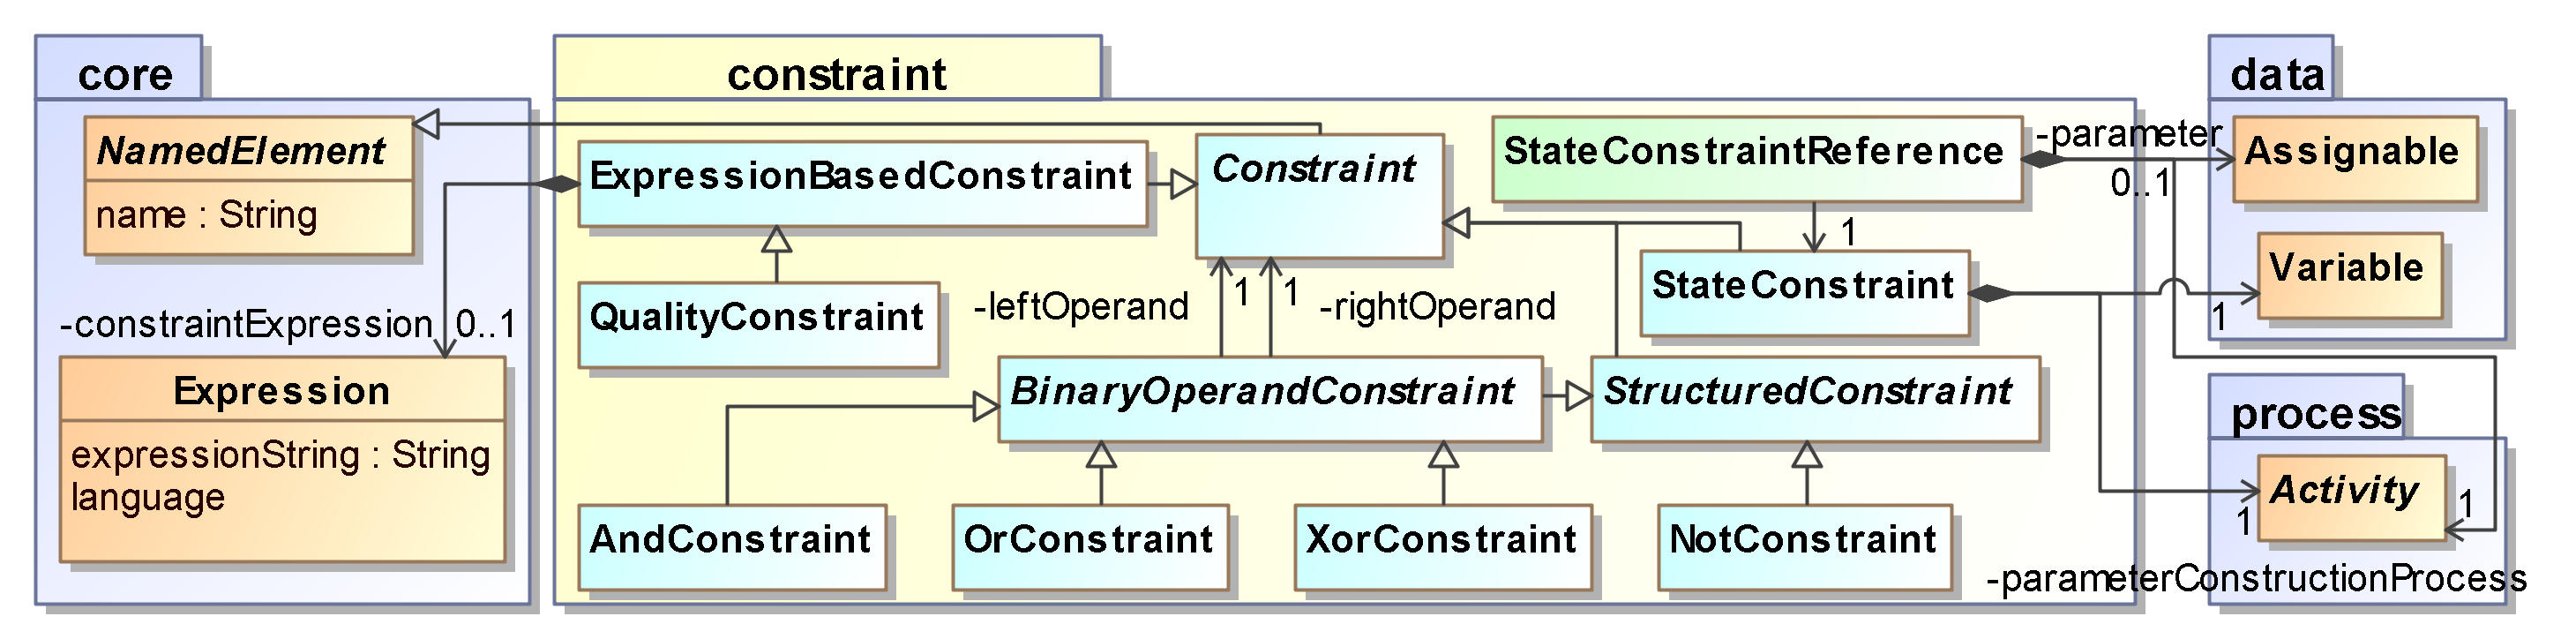
\includegraphics{constraint}
  \caption{The constraint specification elements of URDAD}
  \label{fig:metamodel}
\end{figure}

The constraints provides the concept of re-usable constraints,  module enables one to specify stand-alone, reusable constraints. These constraints can be re-used across, for example, pre- and post-conditions, \verb+if+ and \verb+while+ statements. 
The URDAD-DSL also adds the concept of logical operators in order to assemble higher-level constraints from lower level constraints.


%--------------------------

\subsection{Services contracts}

\begin{figure}
  \centering
  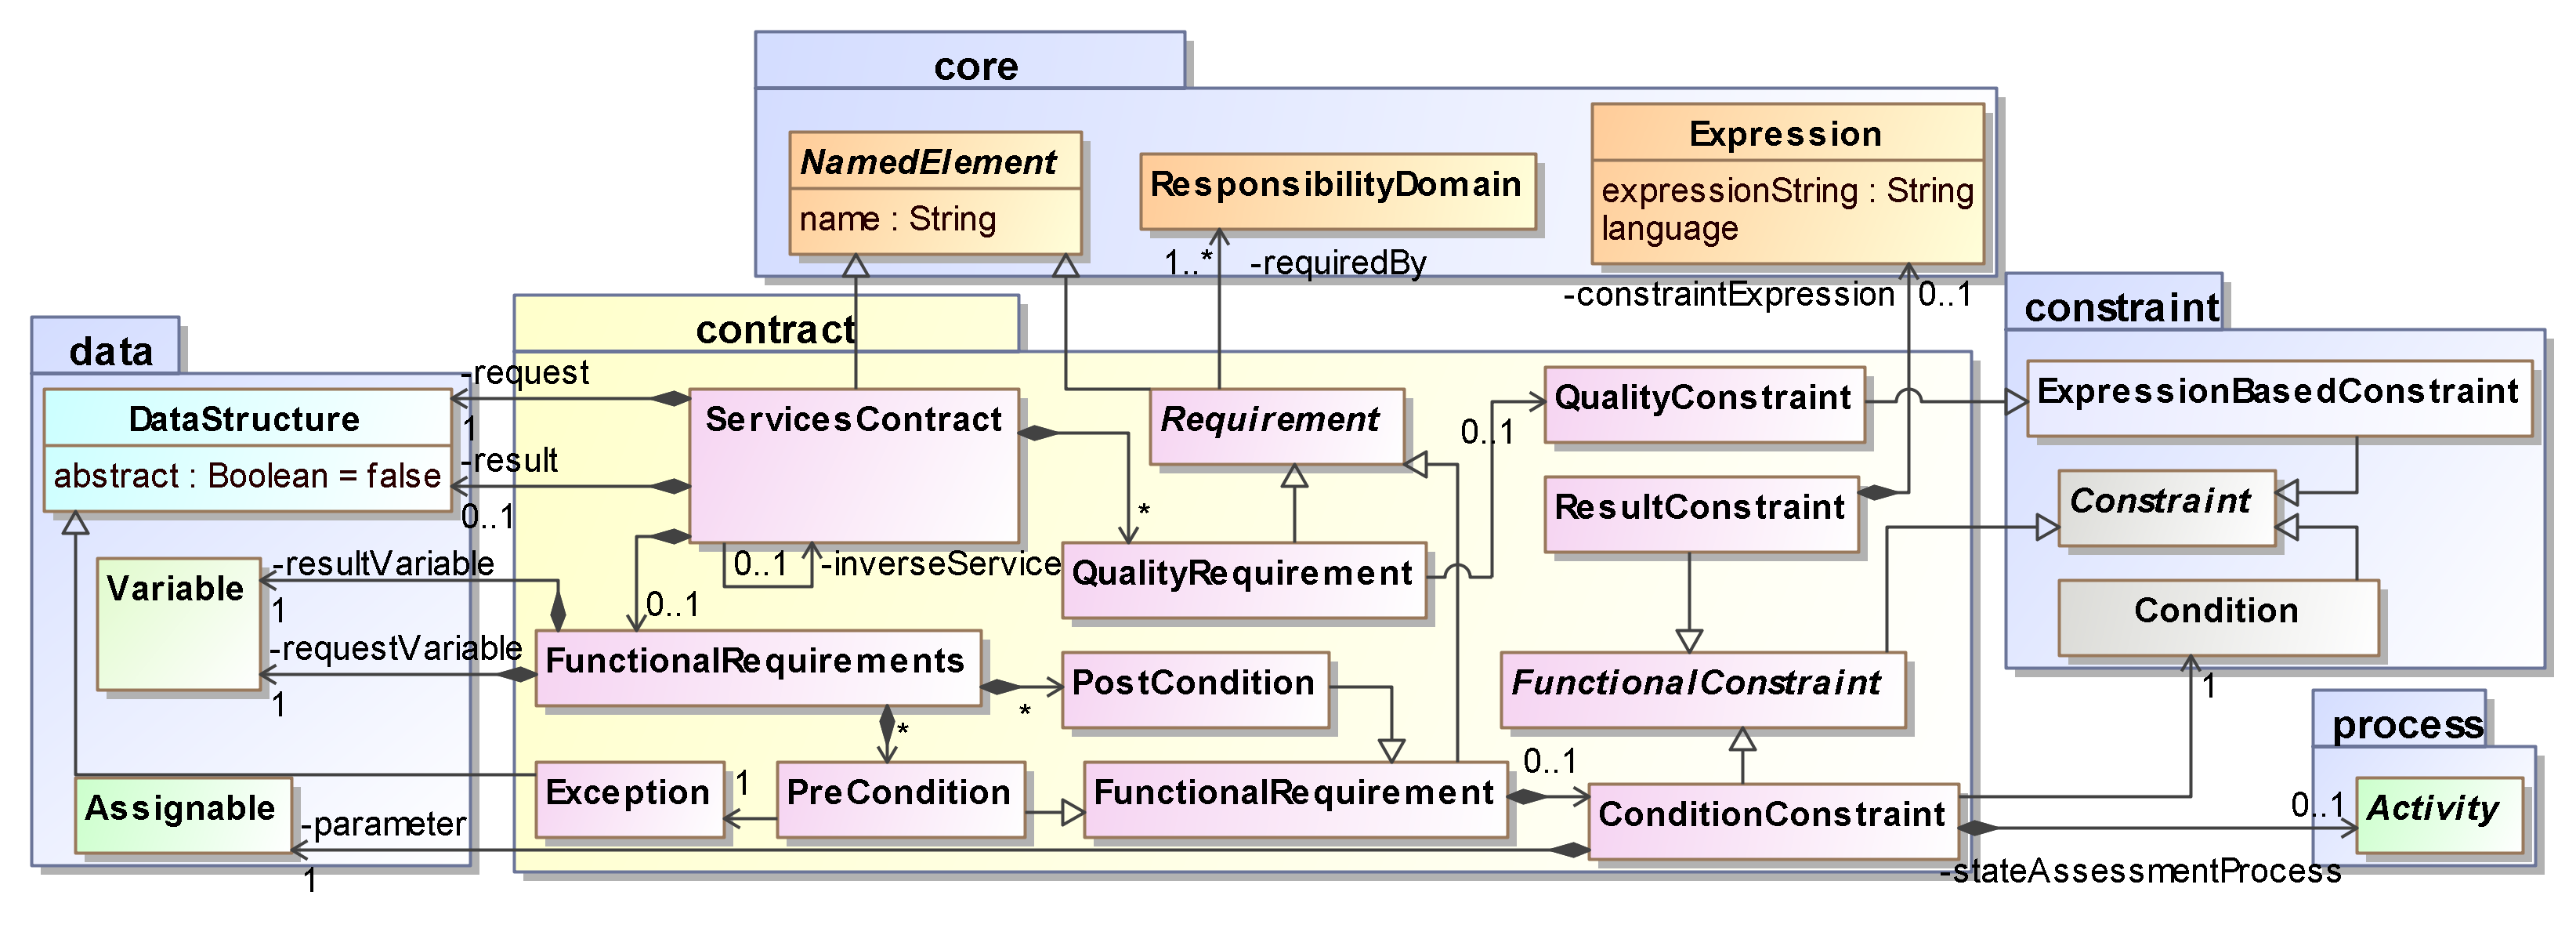
\includegraphics{contract}
  \caption{The contract specification elements of URDAD}
  \label{fig:metamodel}
\end{figure}

%--------------------------

\subsection{Data structures}

\begin{figure}
  \centering
  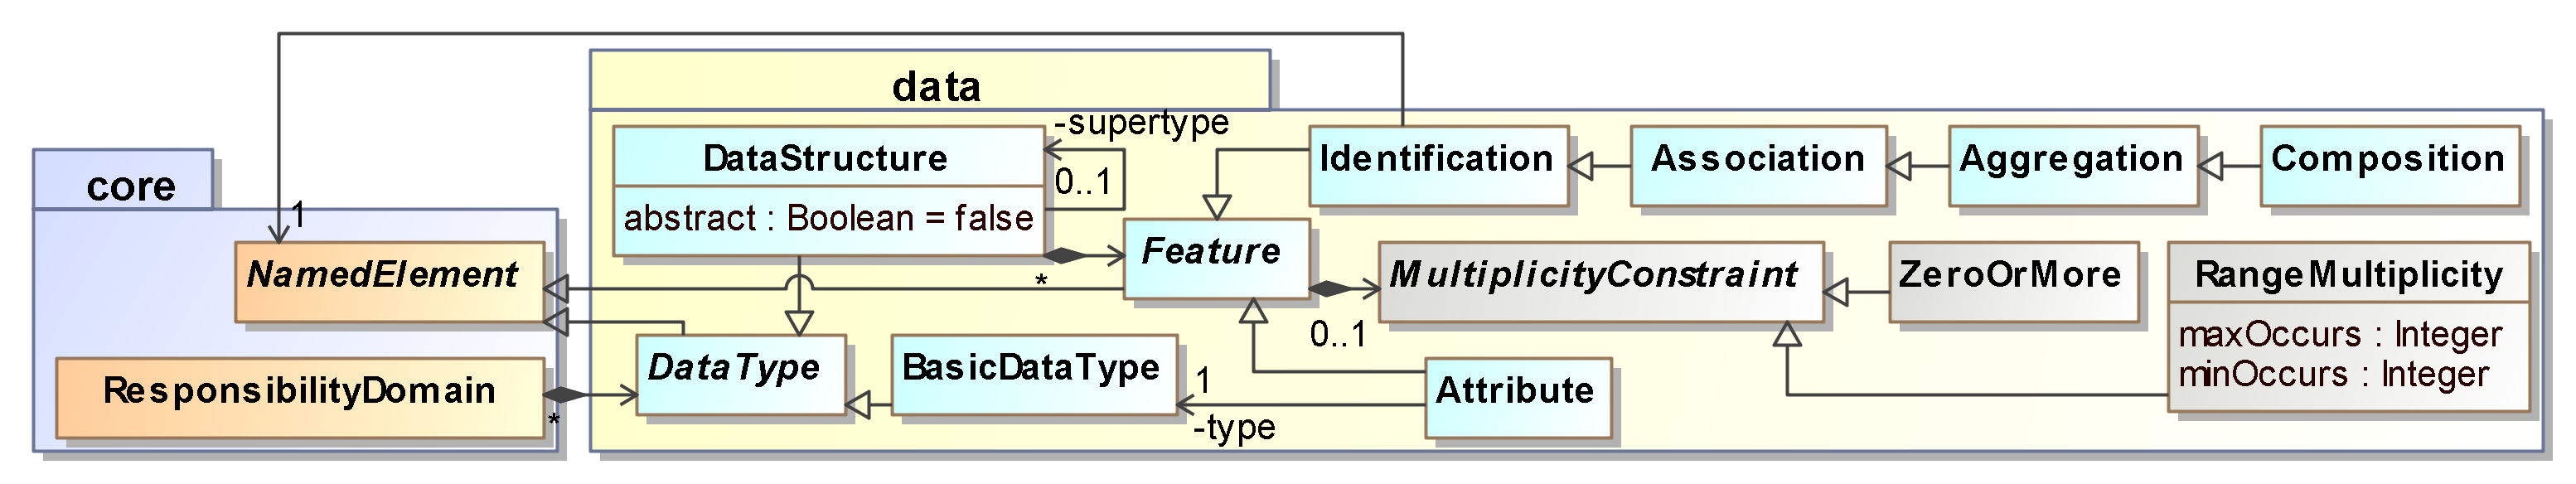
\includegraphics{data}
  \caption{The data definition elements of URDAD}
  \label{fig:metamodel}
\end{figure}




%--------------------------

\subsubsection{Processes}

An URDAD service is a service from a requirements perspective, i.e. it represents a required service, not a provided service. 


Services represent a cohesive unit of required functionality. They exist to address the functional and quality requirements of their stakeholders. These functional and quality requirements are not restricted to a single service and may be used by other services that share some of the same requirements.

A service is specified as a formalised contract, with explicitly defined requirements. The stakeholders who have a direct or indirect interest in the fulfilment of the service, are related to the service via their requirements. Each service has a service signature. The signature takes the form of an appropriately named service, a single service request object that contains information pertaining to the request and a single result object, which is composed of the information associated with the result of the service execution.

%Fixing of levels of granularity

Levels of granularity are explicitly defined within URDAD. Each service exists at a particular level of granularity, when viewed within the context of its utilisation by other another service that exists at a higher level of granularity.

forAll is equivalent to UML expansion regions


\begin{figure}
  \centering
  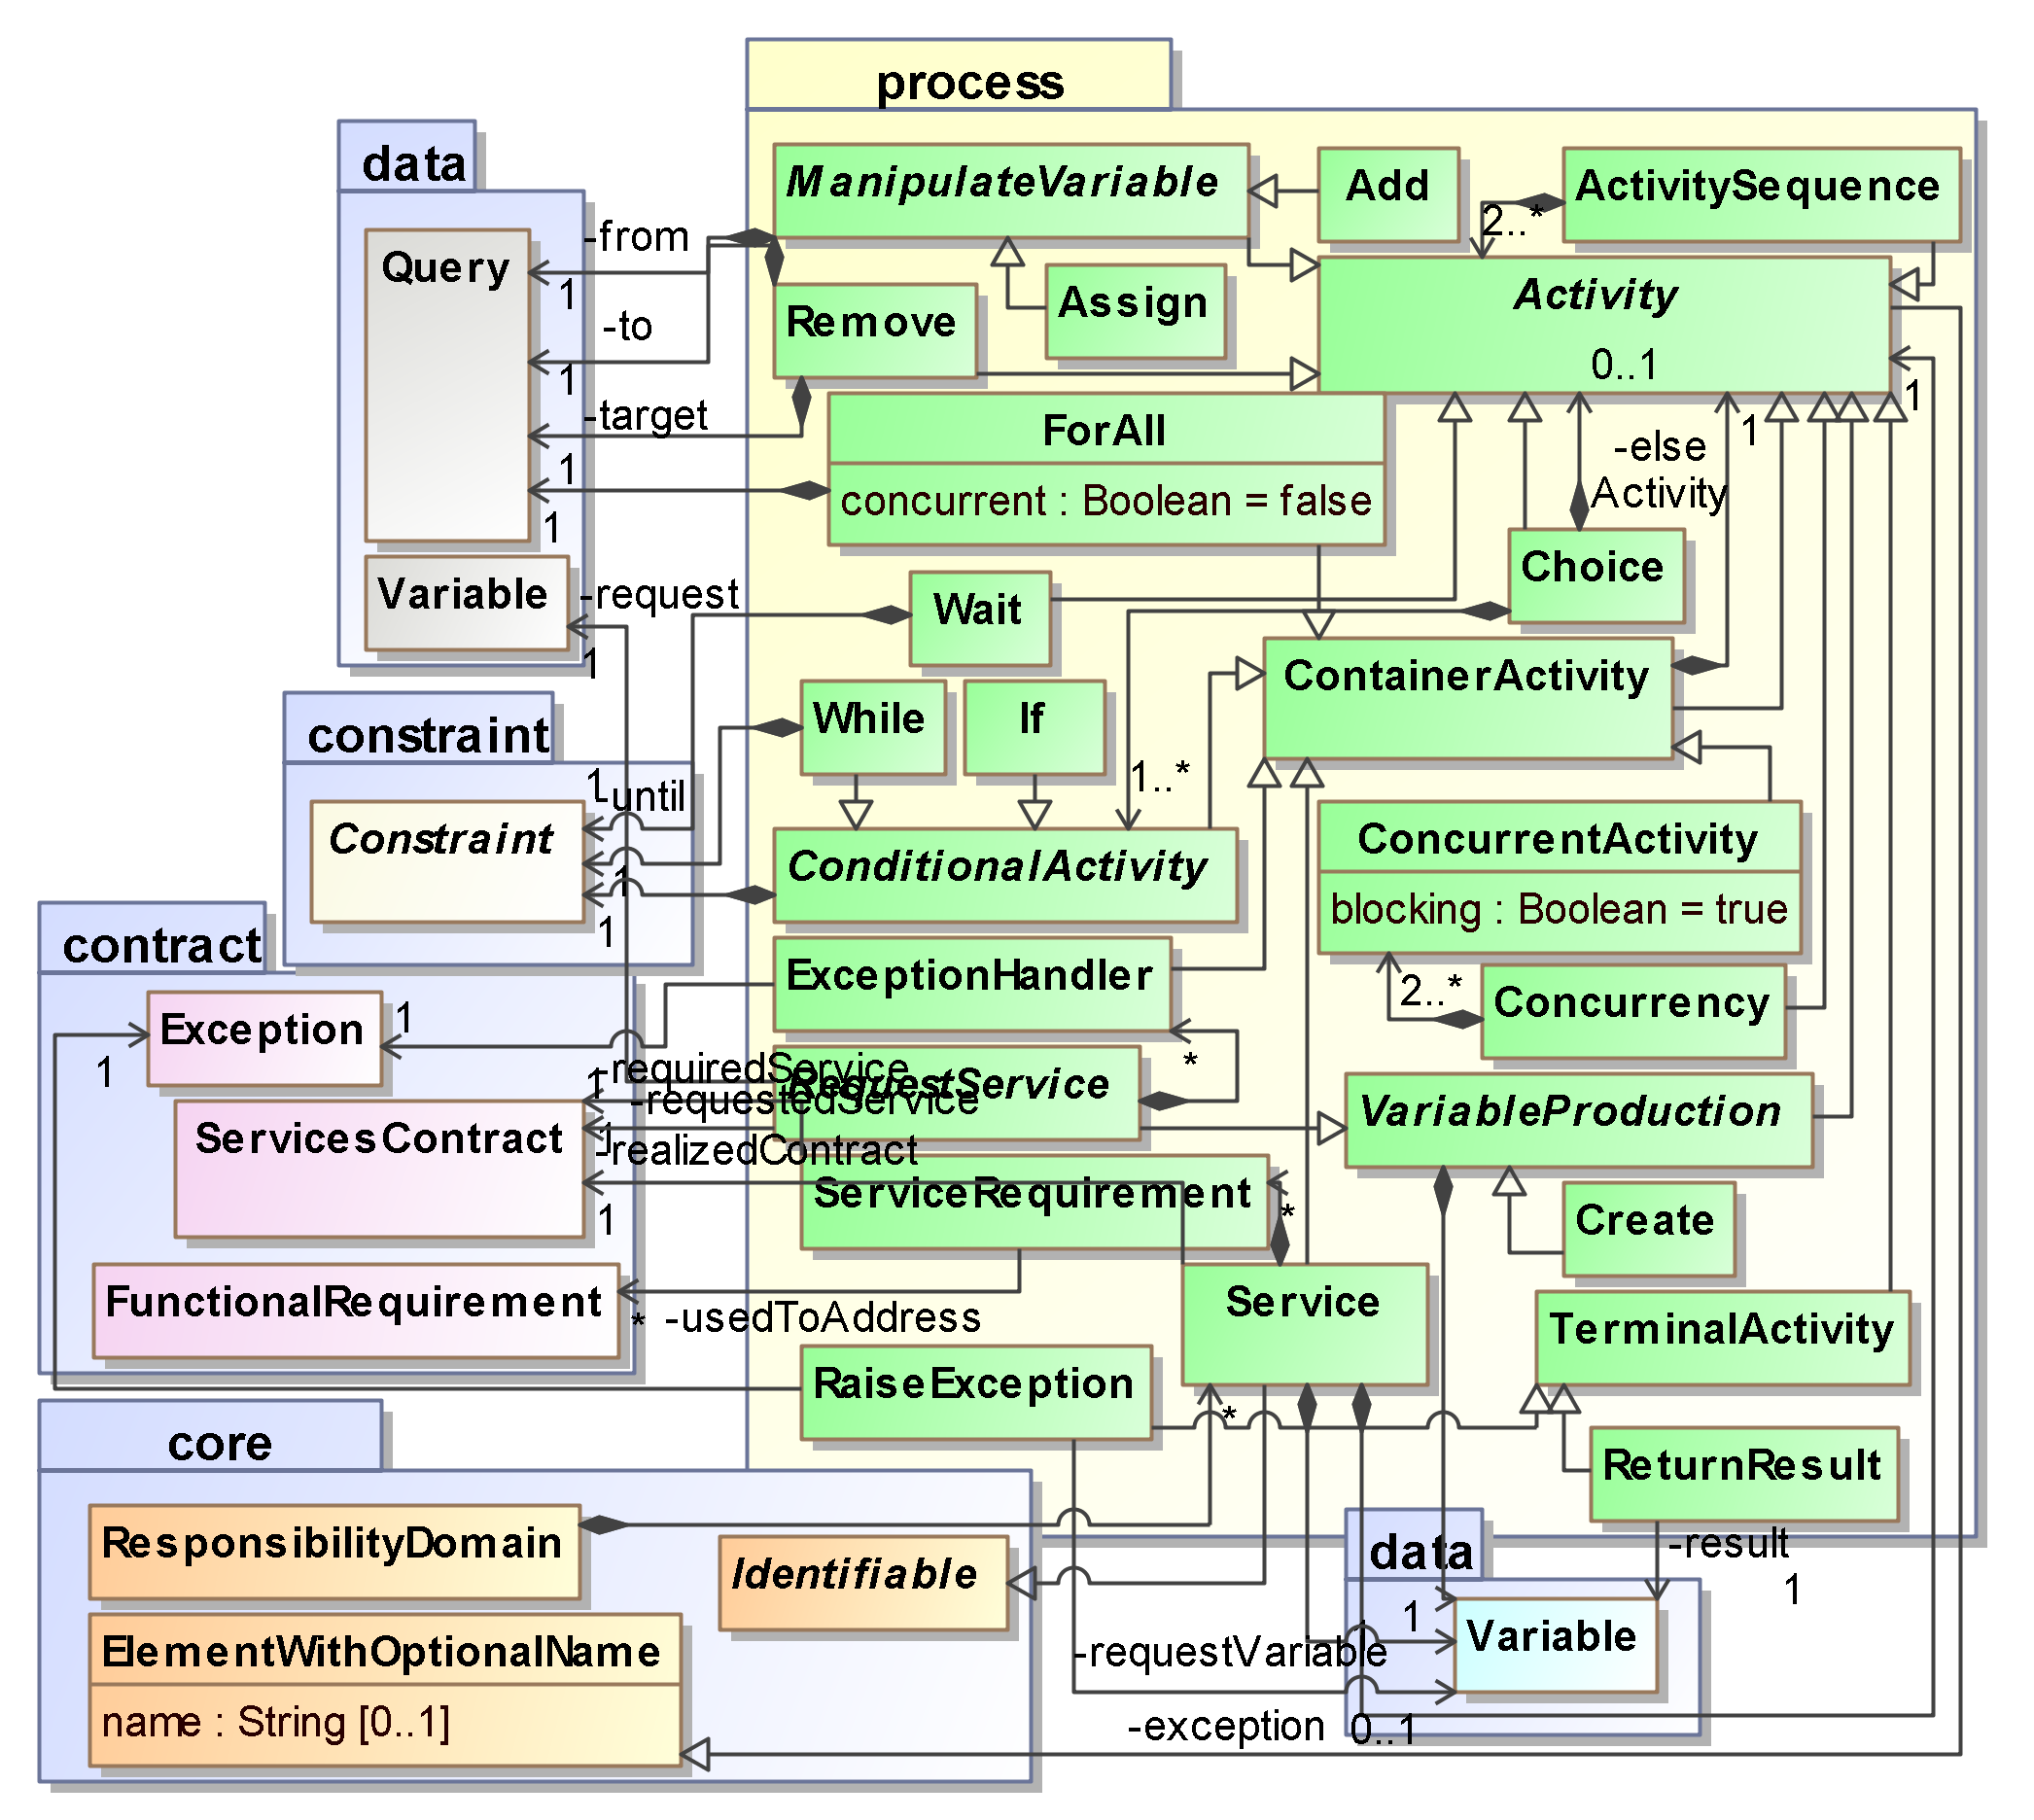
\includegraphics{process}
  \caption{The process definition elements of URDAD}
  \label{fig:metamodel}
\end{figure}








functional and quality requirements can be reused across services. 

data types and data structures

expressions including constraint expressions

 In practice, service requirements are a way of documenting the required functionality. It does not meanCan plug in different services with appropriate adapter


\subsubsection{Pre- and post-conditions}

A pre-condition represents a condition under which the requested service can be refused. The process executed thus far is rolled back and the requester of the service is informed via an appropriate exception that the service was not provided. 

{\em Craig: Needs to be reworded for clarity and eliminate of the phrase 'flown in'}
The refusal of the service may be either due to information within the process (the original requests or any other information which has flown into the process via results from previous service requests), or due to the state of the environment. In the former case the pre-condition itself is specified as an OCL constraint on the information objects available to the process. In the latter case the pre-condition is the combination of a service request to obtain information about the environment and a OCL constraint on the results received from the request as well as potentially any other information objects available to the process. For a pre-condition we thus have an optional service requirement together with a constraint.

A post-condition is a condition which must hold after the service has been provided. Since services themselves are stateless, the post-condition can only refer to a change in the environment. URDAD requires that one specifies the requirements for a service which makes those environmental changes and that the post-condition has a dependency on the service. An inverse service may also be specified, which is tasked with reversing the impact the fulfilment of a post-condition has had on its environment, in the event of an error occurring during the execution of the service.

\subsubsection{Process definition}

A process definition is associated with each service and is composed of all the activities that are required to provide the service. Each activity must either be associated with the validation of a pre-condition, or with the fulfilment of a post-condition, through the execution of a lower level service. A single activity may also be simultaneously responsible for both the validation of a pre-condition and fulfilment of a post-condition, through the execution of a single lower level service. Other activities such as concurrent, control and conditional activities are used for process orchestration, while a result activity is responsible for constructing the service's result object, once the process has finished executing. 

An important non-functional requirement of all activities that constitute a service's process, is that each activity must be traceable back to the fulfilment of one or more of the functional requirements. There should be no redundancy and only the functional requirements that are associated with the service should be addressed by the process.

\subsection{Business process design}
- for a service we have pre- and post-conditions - some of these may be conditional
- lower level services either just check a pre-condition or ensure a post-condition
- these lower level post-condition addressing services may themselves have pre-conditions and some \emph{AP: Why only some?} of those pre-conditions may be part of the pre-conditions for the higher level service.

During business process design one
  1. picks the required services to address the post-conditions
  2. Check which of the higher level pre-conditions are not pre-conditions of lower level services and hence not checked by those services which address the post-conditions and sources the appropriate service spec for those remaining pre-conditions.
  3. One then determines the dependencies between the services, e.g., 
    - to assemble the request for service A I require the information provided by service A
    - I should only issue an invoice if I could reserve a seat
  4. This defines an activity sequence with number of activities equal to number of dependency levels.
  5. Within a dependency level, there may be multiple services which do not have dependencies on each other - these can be executed concurrently.
  6. For conditional pre-or post-conditions, the corresponding services need to be requested under the respective conditions.

\subsection{The metamodel}








there are many options for process specification. Even in UML one can use multiple ways of specifying a process including sequence diagrams, activity diagrams and state machined. Our process specification is similar to that of BPEL (both are services oriented). Just that the semantics ties in with the rest of URDAD (services used to address pre/post conditions, service refused on account of a particular precondition not having been met, ...)

Please also refer to the discussion on exceptions above. The URDAD DSL does not lcok into using OCL and leaves the constraint language pluggable. In practice, however, one would currently largely use OCL, and, yes, the formal specification of the pre and post conditions would be encoded in the chosen constraint language.

> Page 8: The use of the terms "process", "activity", and "service"
> is confusing. A diagram may help to make clear the relations.
I will clarify this. A service is a unit of functionality for which there is a contract. A process is a special activity which realizes a service - i.e. a particular way of providing that unit of functionality. An activity is either the process as a whole or a process component. The concepts should be clear from the diagrammatic representation of the metamodel (attached and in Wiki - will be fed into paper).

The URDAD-DSL is a simpler language to encode an URDAD model in resulting in lower model complexity, faster model encoding and reduced errors around missing links". For example, in a UML encoding the BA has to add the link connecting a use case with a service (otherwise they are not connected in UML, even though UML says a use case is a service which generates value to the user, there is no physical linkage in UML, linkage between functional requirements and pre/post-conditions, enforcing that the only exception which may be raised is one of the exceptions associated with one of the preconditions of the service, ..., and that a process can only end by either returning the deliverable or raising one of the allowed exceptions, etc etc. All that linkage is in the URDAD DSL)





Domain experts collaborate to specify domain model

Discuss recursive nature of URDAD, i.e. how URDAD can be used to design itself but refer to quality paper - feed that into quality paper.

On the other hand, there is a recursive aspect to the URDAD method. If
we view the process of performing the requirements elicitation and
process design for  a level of granularity as a service with defined
inputs and outputs, pre and post-conditions. That service will call
itself for the lower level services, performing the same activities at
the next lower level of granularity. That is of course only required for
those lower level services which do not yet exist. In this sense the
URDAD methodology is recursive, but the URDAD metamodel itself is more
fractal than recursive.

Another interesting aspect which I would like to cover in the quality
paper is that one must be able to design URDAD using URDAD for URDAD to
be a consistent methodology (this is independent of the metamodel and
hence not in the metamodel paper). URDAD is meant to be a methodology of
technology neutral analysis and process design of services. If we use
URDAD to analyze the requirements for the service of doing the
technology neutral analysis and design, we should end up with a process
which is URDAD. Otherwise URDAD is not internally consistent.


Explain responsibility domain

An exception is the notification to a user/client that the requested service is not going to be provided. An exception is always associated with one of the preconditions of a service. If all preconditions are met, the service must be provided as per contract, otherwise there is an error. Thus, if I withdraw cash and my account is in its current state, I might get an InsufficientFundsException - there is no error, just a notification that the withdrawel service is not provided because one of the preconditions of the service is not met. However, if it calculates the service fees and there is a divide by zero or the DB is down, then there is an error which needs to be fixed. Exceptions are just as relevant at the business level as at the technical level.





\begin{itemize}

	\item URDAD META MODEL JUSTIFICATION
	\begin{itemize}
		\item In an effort to formalise URDAD, there exists a need for the formal specification of URDAD's semantics. 
		\item The concepts and rules associated with the use of the URDAD methodology must be clearly defined.
		\item The creation of an URDAD metamodel will assist with the formal definition of URDAD's semantics.
		\item Define Metamodeling
		\item Models versus metamodels. Matter of perception. Discuss levels of abstraction. (One particular metamodel may be considered to be an instance model of another more abstract metamodel.) 
		\item A metamodel represents a level of abstraction.
		\item	Metamodels are closely related to ontologies. (Concept definition, depiction, including relationships between concepts) DISCUSS
		\item While the concepts associated with URDAD are independent of any particular technology or organisation, URDAD is currently used to produce Platform Independent Models (PIMs) as envisaged in Model Driven Architecture (MDA), the Object Management Group's (OMG) approach to Model Driven Engineering. 
		\item PIMs are independent representations of processes, which may or may not be implemented as a software system. They are used to depict the functional requirements of a system. Once all non-functional requirements have been taken into consideration and an appropriate implementation environment has been selected, PIMs can be used to create Platform Specific Models (PSM) through a process of model transformation and refinement. Unlike PIMs, PSMs are inseparable from the actual technology platforms that will be used to implement the system.
		\item	Historically UML has been used to encode URDAD models. 
		\item	UML was a natural selection considering that it represents a standards-based modelling language that is managed by the OMG.
		\item	Unfortunately encoding the URDAD model in UML is not a trivial exercise.
		\item	It is difficult to ensure that the model is encoded in a consistent manner and it requires a strong discipline in the usage of UML.
		\item For example, actors are used to represent the stakeholders in UML use case diagrams. URDAD prescribes the use of interfaces to depict the roles fulfilled by stakeholders.
		\item For each service URDAD requires that there is a clear linkage between the service's stakeholders and their functional and quality requirements. (REF URDAD paper)
		\item An URDAD UML profile was created in order to help ensure that URDAD UML models are consistently encoded.
		\item For example, the URDAD profile introduced a <<requires>> dependency which facilitated the linkage between a service's stakeholders and their requirements.
		\item However, while this profile has helped improve the quality and consistency of URDAD models encoded in UML, the process is still error prone and unintuitive.
		\item Domain experts tasked with creating URDAD UML models are forced to add a range of mundane relationships and stereotypes in order to accurately capture URDAD's semantics. 
		\item It is also not trivial to capture certain aspects of URDAD's semantics in UML, even with the assistance for a UML profile. (Examples?)
		\item The creation of an URDAD metamodel attempts to address these issues.
		\item Depending on the manner in which the metamodel is encoded, URDAD models that conform to the metamodel will require substantially less manual validation. These models will also hopefully be less complex, especially if tools are developed to support the creation of these models.
	\end{itemize}

	\item CONCEPTS THAT DEFINE URDAD'S METAMODEL
		\begin{itemize}
			\item The URDAD metamodel and the semantics it seeks to define, are independent of its physical encoding.
			\item URDAD's metamodel can be encoded in more than one format.
			\item When selecting a mechanism to encode the metamodel, it is critical that URDAD semantics are represented in their entirety. If this is not the case one could argue that the encoded metamodel does not truly represent URDAD.
{\em Fritz: What is meant by this?}
			\item The fundamental concepts \emph{AP: Are there more?} that define the URDAD metamodel are as follows:
			\begin{itemize}

				\item THE MODEL
					\begin{itemize}
						\item Represents the requirements model instance and it constituents
						\item A model represents the formal definition of requirements for a problem domain, modeled as services within responsibility domains, where each service is constrained by the functional and quality requirements of its stakeholders. The stakeholders are themselves represented as responsibility domains.
					\end{itemize}
					
				\item RESPONSIBILITY DOMAINS
					\begin{itemize}
						\item Represents a logical grouping of elements within a model, where each element belongs to the responsibility domain.
						\item Similar to the concept of packaging, but conceptually more consistent with the responsibility driven nature of URDAD.
						\item Responsibility domains also provide a consistent mechanism of depicting the roles/stakeholders within the model.
						\item Responsibility domains must only be composed of data structures, services, requirements and other responsibility domains.
						\item Each role is associated with a cohesive list of responsibilities.
						\item The introduction of the concept of a responsibility domain eliminates the need for the separate definition of a services contract, which is traditionally used to group logically related services. Services are now grouped by the responsibility domain within which they reside.
						\item In the tradition of namespaces each element within a responsibility domain is uniquely identified by its name appended to the fully qualified name of the domain itself.
					\end{itemize}
					
					
					
					
				\item SERVICES
					\item Each service exists to realise a use case 
{\em Fritz: at some level of granularity the user might be a higher level service, maybe we want to avoid the use case vs service mess and focus on using services} and fulfil the requirements of its stakeholders.
					\item Users of a service are also represented as stakeholders.
					\item Services represent a level of granularity. Each level of granularity can be regarded as a level of abstraction.
					\item Requirements exist at a particular level of granularity, and are themselves decomposed further across subsequent lower levels of granularity.
					\item There are two forms of requirements that a service seeks to address namely functional and quality requirements.
					\item It is important to note that both functional and quality requirements are not restricted to a single service. There exists the reality that several services may have requirements in common.
					\item URDAD does not address any non-functional requirements other than the non-functional requirements of the requirements themselves. For example, requirements should be easy to maintain. Requirements should exhibit principles of good design, such as decomposition across layers of granularity, single responsibility, loose coupling and high cohesiveness.
					\item Each service is represented as a formalised contract, with explicit pre and post conditions that seek to address the functional requirements of the service.
					\item Pre-conditions represent the conditions under which the service may legally be refused. A pre-condition's existence must be justified by a tangible functional requirement. 
					\item A pre-condition is contractually obligated to raise an exception if it is not fulfilled. This exception must be clearly specified on the service contract.
					\item Post-conditions represent the conditions that must hold true if all the pre-conditions have be fulfilled and the service is complete.
			
			
			
					\item Unless the service has been sourced from the environment, it must be possible to verify whether each post-condition has been fulfilled. (VERIFY THIS STATEMENT)
					\item The fulfilment of a post condition may have a lasting impact on the state of the environment. Inverse services may be associated with each post-condition. These services are responsible for reversing the effects the post-condition had on the environment and returning the environment to its original state, in the event of an error occurring during the execution of the service.
					\item Associated with each service there exists a process definition that is composed of all the activities that are required to provide the service. Each activity must either directly or directly be associated with:
						\begin{itemize}
							\item The validation of a pre-condition through the execution of a lower level service.
							\item The fulfilment of a post-condition through the execution of a lower level service.
							\item The simultaneous validation of a pre-condition and fulfilment of a post-condition; through the execution of a common lower level service.
							\item The construction of the service result
						\end{itemize}
					\item The process defines the logical orchestration of the activities that are required to provide the service.
					\item The lower level services utilised by each activity constitute the next level of granularity, when considered in the context of the particular service in question.
					\item All activities within a process must directly address one or more of the functional requirements associated with the service.
					\item No activities should exist that do not address functional requirements.
					\item An important non-functional requirement of all activities that constitute a service, is that each activity must be able to be traced back to the fulfilment of a functional requirement. There should be no redundancy.
					\item Each service has a consistent service signature. The signature takes the form of an appropriately named service, a single service request object that contains detailed information pertaining to the request and a single result object, which is composed of the information associated with the result of the service execution.
					\item Traceability is one of the essential characteristics of the service contract and its process definition. Traceability is realised as follows:
						\begin{itemize}
							\item Ensuring that activities only exist to address a pre-condition, a post-condition or both a pre-condition and a post-condition simultaneously.
							\item Associating each functional requirement with one or more stakeholder's represented as responsibility domains.
							\item Ensuring that a service addresses all functional requirements and only the relevant functional requirements.
						\end{itemize}
			\end{itemize}
		\end{itemize}
		

		
		
	
	\item METAMODEL ENCODING OPTIONS
		\begin{itemize}
				\item There are many languages and approaches that can be used to encode the URDAD metamodel. 
				\item It is important that the advantages and disadvantages of each encoding option are carefully taken into consideration.
				\item Regardless of the encoding option that is ultimately selected, URDAD's semantics must be able to be represented in their entirety.
				\item Each encoding may differ in the way in which URDAD's semantics are depicted.				
				\item (INSERT REF - Quality in Model-Driven Engineering) argues that model quality is determined by five aspects. The modeling language and tools used to define the model, the modeling process itself, techniques used to assure quality and the relative experience of the individuals tasked with building the model.
				\item An encoding option should be assessed according to these five aspects.
				\item Three encoding options have been considered. Encoding options are not mutually exclusive and several may be concurrently utilised if each offers its own unique advantages. For example, one particular encoding option may make it easier to represent semantics and reason about the model, while another encoding option may be aligned with standards and offer extensive tool support for model tool smiths and practitioners. 
				\item Currently three encoding options have been taken into consideration.
				\item The first option is to attempt to improve the UML encoding of URDAD. While this will always be an option worth considering, it was quickly discarded for the reasons already mentioned in this paper.
				\item Another encoding option that has been considered is the encoding of the URDAD metamodel in a knowledge representation language such as the Web Ontology Language (OWL) or more specifically OWL-DL one of OWL's sub languages. There are many benefits associated with this option... (ELABORATE)
				\item The third opinion and the encoding which represents the focus of this paper is to encode the URDAD metamodel using the Eclipse Modeling Framework's (EMF) Ecore metamodel. 
				\item It is possible to capture URDAD's metamodel by extending the Ecore metamodel and introducing URDAD's semantics.
				\item The Eclipse 
				
		TODO COMPLETE...		

		Discuss the tool support
		Discuss Ecore and in particular the Eclipse Modeling Project's alignment with the OMG standards.
			Natural selection considering URDAD current alignment with the OMG's MDA
			Ecore <-> EMOF
			OCL
			QVT
		M2T
		Textual and graphical concrete syntaxes (XText and EMF Text)
		Model Validation
		IDE environment - services offered (syntax checking etc)
		
			\item One may consider the formalisation and encoding of URDAD's metamodel to be an attempt to establish a Domain Specific Language (DSL) for URDAD by defining its abstract syntax.
			
		\end{itemize}
	
	\item THE ECORE METAMODEL ENCODING 
	
	TODO COMPLETE...
	
	Discuss how the URDAD metamodel is realised in Ecore
		
	\item OUTSTANDING ISSUES AND POSSIBLE IMPROVEMENTS TO THE ECORE METAMODEL
	
	TODO COMPLETE...
		
\end{itemize}

\section{Assessing the URDAD metamodel \label{sec:metamodelAssessment}}



%-------------------------------------------------------------------------------------

\subsection{Core metamodel integrity assessment}


\begin{itemize}
  \item Check that no classes unsatisfiable
  \item Check consistency of OCL constraints
  \item Redundency checks (redundent classes, redundent attributes and properties) redundend constraints
\end{itemize}

%-------------------------------------------------------------------------------------

\subsection{Assessing model qualities}

\begin{itemize}
  \item Comparing complexity of URDAD-DSL and UML encodings of URDAD model
    \begin{itemize}
     \item UML model requires much more model elements to encode URDAD semantics.
    \end{itemize}
  \item Assessing traceability (\cite{dick_design_2005} - see notes on Zotero entry)
  \item Completeness checks
(What does completeness mean - That only technical information needs to be provided and that the full requirements
from a business perspective are specified across levels of granularity.)
    \begin{itemize}
     \item all OCL constraints for decision conditions specified
     \item all OCL constraints for pre and post-conditions specified
     \item All required request and result fields all specified either via OCL constraints 
	or by default values.
    \end{itemize}
  \item Check that process addresses all functional requirements and nothing but the functional requirements.
\end{itemize}

%-------------------------------------------------------------------------------------

\subsection{Sufficiency}

An URDAD model is meant to be able to absorb the information required for performing implementation mappings, generating service tests, and
requirements traceability.


Jeremy Dick \cite{dick_design_2005} emphasizes the importance of traceability need for traceability across levels of granularity

- traceability generally important in design (not only software)

- traceability links can be enriched through rationale sematics (URDAD: requiredBy, requiredService, ...)

- include sufficiency and necessity, i.e. are all requirements met and are all design elements necessary/required to realize requirements

- identify immediate impact point, calculate potential impact tree, prune impact tree

Ramesh et al\. \cite{ramesh_toward_2001} identify 4 core traceability link types including (i) {\em satisfaction links} (ensuring that requirements are satisfied by system), (ii) \emph{evolutional links (document inputs resulting in changes to objects and resulting changes)

  3. Rationale links (why is this required, use instead requires by)

  4. Dependency links (from model reflection: dependency between services and so on)
%-------------------------------------------------------------------------------------

\subsection{Usability assessment (potentially an empirical study)}

\begin{itemize}
 \item Have 2 groups doing URDAD modeling, one using UML encoding and UML tools and one using URDAD encoding.
 \item Assess relative productivity, error densities and completeness of the two resultant models 
\end{itemize}



\section{Related work \label{sec:relatedWork}}

The URDAD methodology provides a services-oriented methodology for generating a semi-formal analysis and design model representing MDA's PIM and supporting test and implementation generation. \cite{iacob_model-driven_2008} discuss an alternative approach. Business Rules are specified using OMG's {\em Semantics for Business Vocabulary and Rules} (SBVR) to service specification and orchestration and BPEL process specifications are generated using MDA tools. Processes are assembled from services which are related to business rules. This is similar to our satisfiability links specifying the services used to realize the different functional requirements.

The URDAD DSL allows for the specification of textual and graphical grammars through which the URDAD model is populated. An alternative approach is to define a separate metamodel for the use case narrative and to transform the narrative model requirements model \cite{hoffmann_towards_2009,osis_transforming_2010}. This approach introduces the complexities of having to transform from the narrative to the UML model and requires extensive consistency checks between the narrative and the UML models.

\cite{asnina_computation_2010} stress the need of modelling in the problem domain as well the benefits of accumulating requirements within a single model. Services are grouped into feature sets which are related to responsibility domains. Functional requirements are decomposed across levels of granularity and higher level processes are orchestrated across lower level services. They define the notion of functionals with cause and effect which can be related to the concept of a services contract. In addition they provide a {\em topological functional model} (TFM) for mapping technology neutral service requirements onto available concrete services pool. The TFM is independent of the modelling technique and can be applied to an URDAD model. 

In the {\em Requirements Driven Design Automation} methodology (RDDA) \cite{cardei_model_2008} one encodes requirements specifications in SYSML diagrams. The SYSML model is enriched with semantic descriptions after which the model is transformed to the {\em One Pass to Production} (OPP) design language, the ODL. ODL is an OWL based ontology from which the requirements are validated for consistency and completeness. The approach is, however, structure focused with little emphasis on services contracts and recursive orchestration of higher level services from lower level services.


\section{Conclusions and outlook}

In this paper we identified the stakeholders in the analysis and design methodology and the resultant requirements and technology neutral process design model and their quality requirements. We related these quality requirements to quality drivers and measures which can be applied within a services-oriented approach. We then identified that subset of quality drivers which has been embedded within the URDAD process and pointed out how some of these are enforced by the URDAD metamodel.

One of the practical benefits of the URDAD methodology is that it assists requirements engineers to make the paradigm shift\cite{haines_impact_2007} to defining stand-alone services contracts and to assemble processess from abstract, reusable, stateless services with the concrete service providers either selected during the implementation mapping phase or alternatively provided by the execution environment through mechanisms like real-time service provider selection and dependency injection.

Future work includes the specification of a graphical grammar making the domain specific language for URDAD accessible to requirements engineers like business analysts and the specification and development of quality assessment tools which can be used to either report quality measures or provide real time quality guidelines to modelers.

\section{Acknowledgements}
We thank the National Research Foundation (NRF) of South Africa for the financial support. Many thanks also to {\it Dawid Loubser} for some fruitful discussions on the topic of this paper.


\bibliographystyle{abbrv}
\bibliography{../../bibliography}

\end{document}